% 20120531-103842-104143
% A-7.0/W32.3

\section{A-7.0/W32.3 - 160 krpm}
\label[secinapp]{sec:awp-exp-details-A-7.0/W32.3}

This test has been performed on May 31\th{} 2012, between 10:38:42 and
19:41:43.

\begin{figure}[htbp]
  \centering
  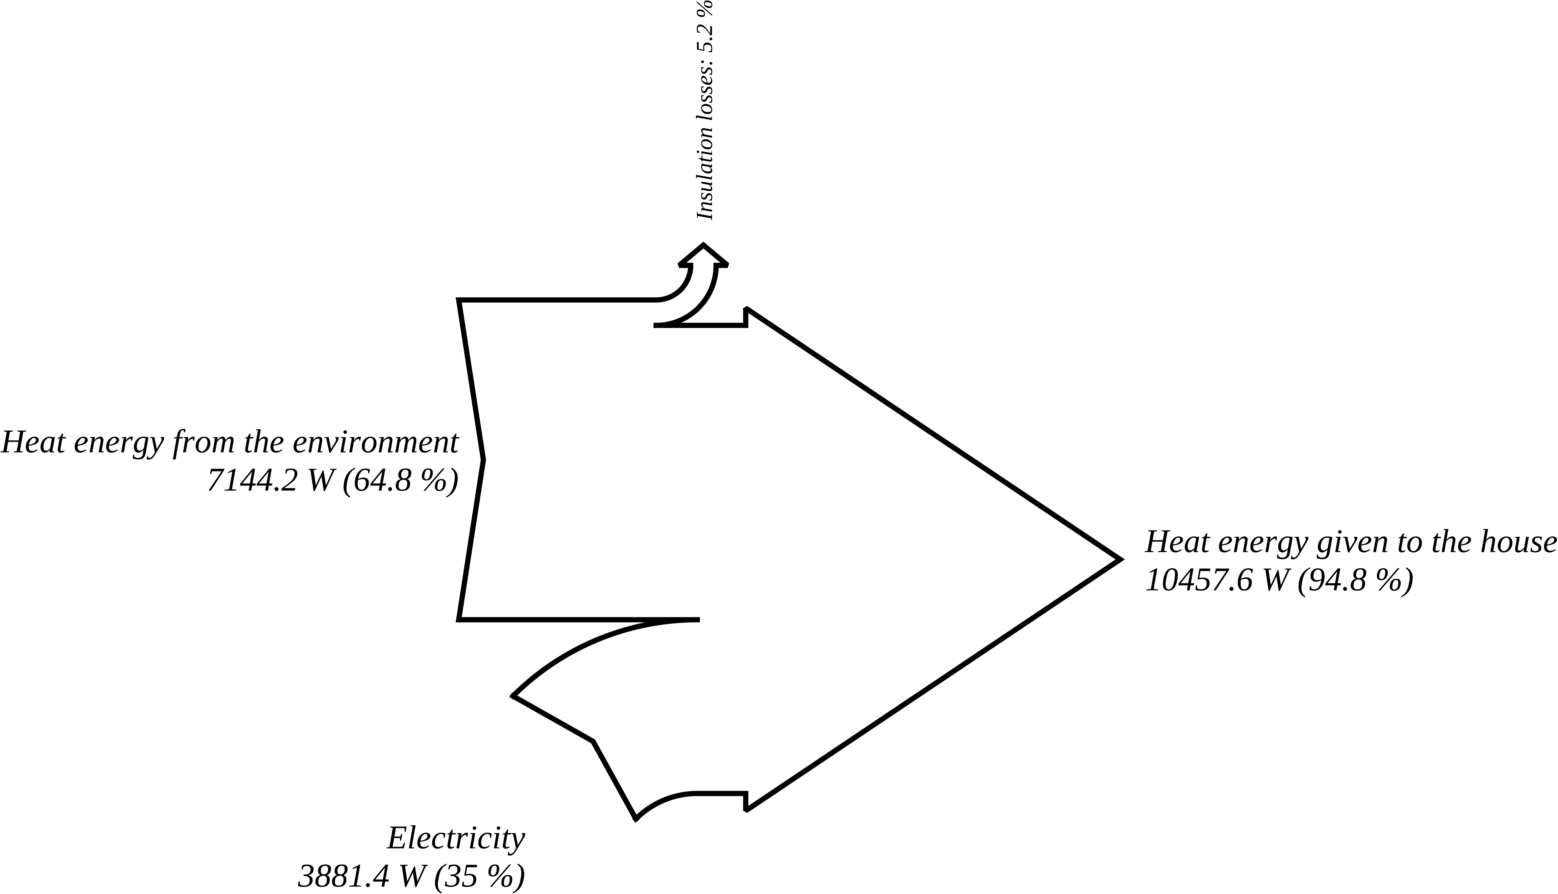
\includegraphics[width=0.7\textwidth]{awp-energy-sankey-awp-20120531-103842-104143}
  \caption{A-7.0/W32.3 -- Sankey diagram for heat pump energy balance (internal frontier)}
  \label{fig:awp-A-7.0/W32.3-sankey-energy}
\end{figure}


\begin{figure}[htbp]
  \centering
  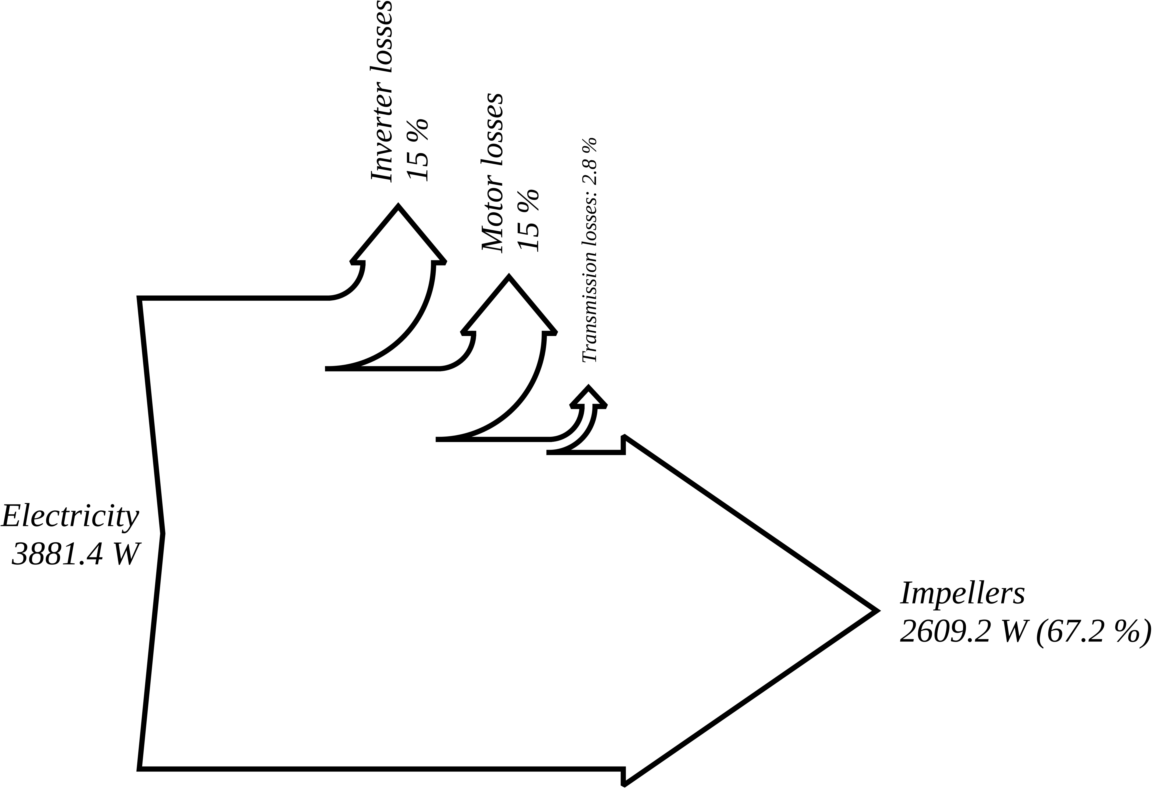
\includegraphics[width=0.7\textwidth]{awp-energy-sankey-cp-20120531-103842-104143}
  \caption{A-7.0/W32.3 -- Sankey diagram for the compressor unit energy balance}
  \label{fig:awp-A-7.0/W32.3-sankey-cp}
\end{figure}

\begin{figure}[htbp]
  \centering
  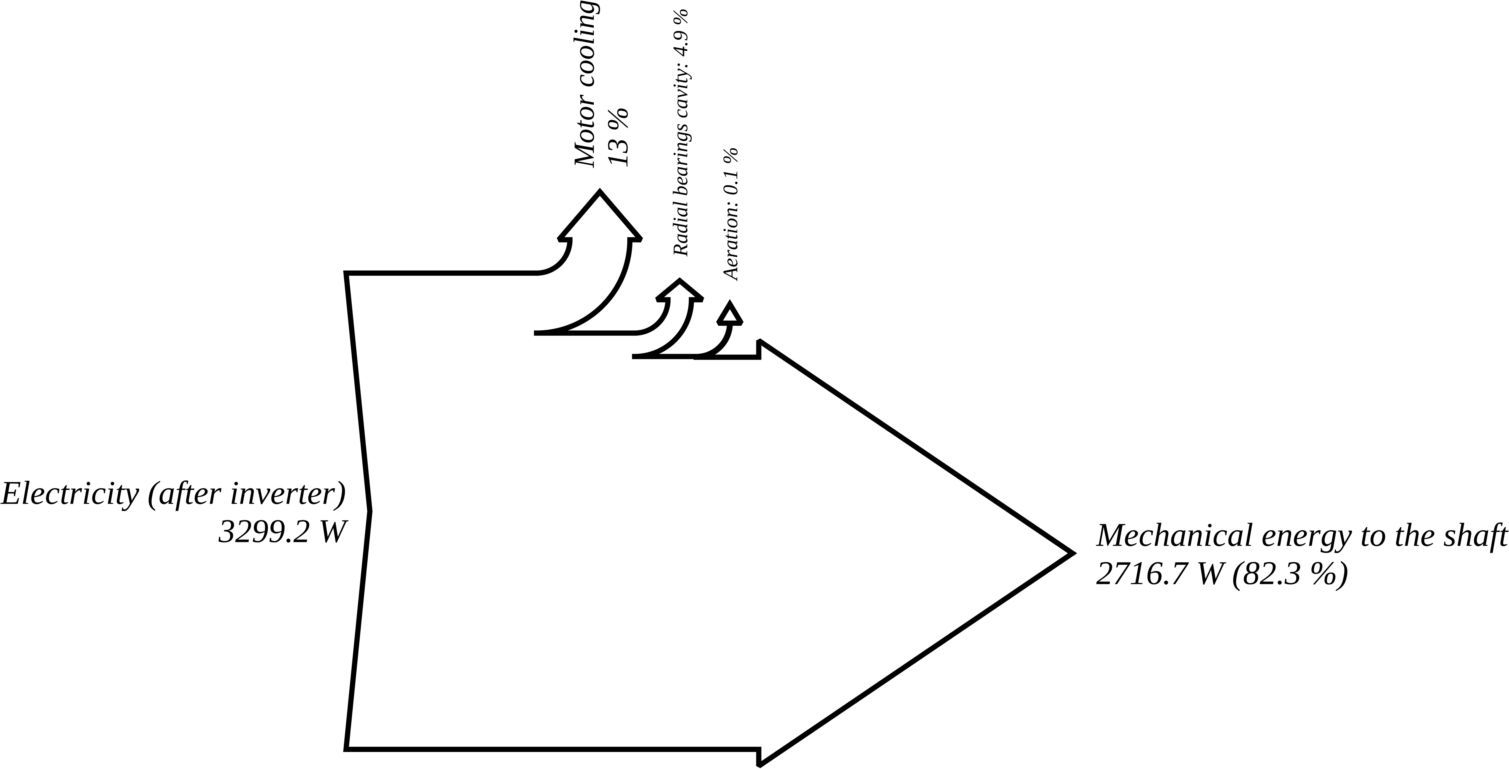
\includegraphics[width=0.7\textwidth]{awp-energy-sankey-motor-20120531-103842-104143}
  \caption{A-7.0/W32.3 -- Sankey diagram for the motor energy balance}
  \label{fig:awp-A-7.0/W32.3-sankey-motor}
\end{figure}

\begin{table}[htbp]
    \footnotesize
    \begin{center}
    \begin{tabular}{llllll}
\toprule
Name & Value / \% & Name & Value / \% & Name & Value / - \\
\midrule
$\eta_{heatpump}$ & $ \num{32.6} \pm \num{0.5} $ & $\eta_{mot}$ & $ \num{82.1} \pm \num{0.3} $ & $\epsilon_h$ & $ \num{2.69} \pm \num{0.03} $\\
$\eta_{cp1}$ & $ \num{63} \pm \num{36} $ & $\eta_{cp2}$ &$ \num{77} \pm \num{22} $ & $\pi_1$ & $ \num{2.440} \pm \num{0.002} $\\
$\eta_{cp1,\,imp}$ & $ \num{63} \pm \num{36} $ & $\eta_{cp2,\,imp}$ & $ \num{80} \pm \num{19} $ & $\pi_2$ & $ \num{2.365} \pm \num{0.001} $\\
$\eta_{cd}$ & $ \num{92} \pm \num{2} $ & $\eta_{ev}$ & $ \num{31} \pm \num{31} $ & $\pi_{1,\,theory}$ & $ \num{3.0} \pm \num{0.2} $\\
$\eta_{trans}$ & $ \num{96.04} \pm \num{0.02} $ & $\eta_{sc}$ & $ \num{2} \pm \num{2} $ & $\pi_{2,\,theory}$ & $ \num{1.922} \pm \num{0.002} $\\
$\eta_{s,\,cp1}$ & $ \num{88} \pm \num{12} $ & $\eta_{s,\,cp2}$ & $ \num{88} \pm \num{12} $ & $\eta_{mot}$ & $\underline{82.34}$ \%\\
$\eta_{s,\,cp1,\,ext}$ & $ \num{94} \pm \num{7} $ & $\eta_{s,\,cp2,\,ext}$ & $ \num{81} \pm \num{19} $ & $\eta_{radial}$ & $ \num{98.54} \pm \num{0.02} $ \%\\
$\eta_{s,\,cp1,\,theory}$ & $ \num{79} \pm \num{2} $ & $\eta_{s,\,cp2,\,theory}$ & $ \num{72.37} \pm \num{0.04} $ & $\eta_{axial}$ & $ \num{97.47} \pm \num{0.02} $ \%\\
\bottomrule
\end{tabular}

  \end{center}
  \caption{A-7.0/W32.3 -- Performance indicators}
\end{table}

\begin{table}[htbp]
  \footnotesize
  \begin{center}
    \begin{tabular}{cccccc}
\toprule
Component & Location & P / \si{\bar} & T / \si{\degreeCelsius} & h / \si{\kilo\joule\per\kilo\gram} & s / \si{\kilo\joule\per\kilo\gram\per\kelvin}\\
\midrule
\multirow{2}{*}{1} & inlet & $ \num{1.502} \pm \num{1.502} $ & $ \num{-11} \pm \num{-11} $ & $ \num{393.226} \pm \num{393.226} $ & $ \num{1.76} \pm \num{1.76} $\\
& outlet & $ \num{3.665} \pm \num{3.665} $ & $ \num{31.1} \pm \num{0.9} $ & $ \num{424.8843} \pm \num{4e+02} $ & $ \num{1.801} \pm \num{1.801} $\\
\midrule
\multirow{2}{*}{2} & inlet & $\pmb{ \num{3.665} \pm \num{3.665} }$ & $\pmb{ \num{8.391} \pm \num{8.391} }$ & $ \num{404.146833} \pm \num{4e+02} $ & $ \num{1.73050} \pm \num{2e+00} $\\
& outlet & $\pmb{ \num{8.668} \pm \num{8.668} }$ & $\pmb{ \num{45.140} \pm \num{45.140} }$ & $ \num{428.511354} \pm \num{4e+02} $ & $ \num{1.75050} \pm \num{2e+00} $\\
\midrule
\multirow{2}{*}{3} & inlet & $\pmb{ \num{8.393} \pm \num{8.393} }$ & $\pmb{ \num{43.907} \pm \num{43.907} }$ & $ \num{427.803896} \pm \num{4e+02} $ & $ \num{1.75050} \pm \num{2e+00} $\\
& outlet & $\pmb{ \num{8.209} \pm \num{8.209} }$ & $\pmb{ \num{31.449} \pm \num{31.449} }$ & $ \num{243.821366} \pm \num{2e+02} $ & $ \num{1.15027} \pm \num{1e+00} $\\
\midrule
\multirow{2}{*}{4} & inlet & $ \num{1.635} \pm \num{1.635} $ & $ \num{-15.1} \pm \num{-15.1} $ & $ \num{227.7822} \pm \num{2e+02} $ & $ \num{1.110} \pm \num{1.110} $\\
& outlet & $\pmb{ \num{1.620} \pm \num{1.620} }$ & $\pmb{ \num{-15.011} \pm \num{-15.011} }$ & $ \num{389.683643} \pm \num{4e+02} $ & $ \num{1.7382} \pm \num{2e+00} $\\
\midrule
\multirow{2}{*}{5} & inlet & $ \num{8.209} \pm \num{8.209} $ & $ \num{31.45} \pm \num{31.45} $ & $ \num{243.82136} \pm \num{2e+02} $ & $ \num{1.1503} \pm \num{1e+00} $\\
& outlet & $ \num{3.665} \pm \num{3.665} $ & $ \num{6.4} \pm \num{0.4} $ & $ \num{243.8214} \pm \num{2e+02} $ & $ \num{1.157} \pm \num{1.157} $\\
\midrule
\multirow{2}{*}{6} & inlet & $ \num{3.665} \pm \num{3.665} $ & $ \num{6} \pm \num{5} $ & $ \num{207.577} \pm \num{207.577} $ & $ \num{1.03} \pm \num{1.03} $\\
& outlet & $ \num{1.886} \pm \num{1.886} $ & $ \num{-11.5} \pm \num{-11.5} $ & $ \num{207.5766} \pm \num{2e+02} $ & $ \num{1.031} \pm \num{1.031} $\\
\midrule
\multirow{2}{*}{7} & inlet & $ \num{1.886} \pm \num{1.886} $ & $ \num{-11.5} \pm \num{-11.5} $ & $ \num{243.8214} \pm \num{2e+02} $ & $ \num{1.169} \pm \num{1.169} $\\
& outlet & $ \num{1.886} \pm \num{1.886} $ & $ \num{-11.5} \pm \num{-11.5} $ & $ \num{288.9457} \pm \num{3e+02} $ & $ \num{1.342} \pm \num{1.342} $\\
\midrule
\multirow{2}{*}{8} & inlet & $\pmb{ \num{3.665} \pm \num{3.665} }$ & $\pmb{ \num{6.357} \pm \num{6.357} }$ & $ \num{402.265796} \pm \num{4e+02} $ & $ \num{1.7238} \pm \num{2e+00} $\\
& outlet & $ \num{3.66} \pm \num{3.66} $ & $ \num{6.4} \pm \num{0.4} $ & $ \num{208.5971} \pm \num{2e+02} $ & $ \num{1.031} \pm \num{1.031} $\\
\midrule
\multirow{2}{*}{9} & inlet & $\pmb{ \num{1.886} \pm \num{1.886} }$ & $\pmb{ \num{-11.547} \pm \num{-11.547} }$ & $ \num{227.782249} \pm \num{2e+02} $ & $ \num{1.10776} \pm \num{1e+00} $\\
& outlet & $ \num{1.635} \pm \num{1.635} $ & $ \num{-15.1} \pm \num{-15.1} $ & $ \num{227.7822} \pm \num{2e+02} $ & $ \num{1.110} \pm \num{1.110} $\\
\midrule
\multirow{2}{*}{10} & inlet & $ \num{8.668} \pm \num{8.668} $ & $ \num{45.1} \pm \num{0.7} $ & $ \num{428.5114} \pm \num{4e+02} $ & $ \num{1.751} \pm \num{1.751} $\\
& outlet & $ \num{3.665} \pm \num{3.665} $ & $ \num{128} \pm \num{88} $ & $ \num{518.04} \pm \num{0.09} $ & $ \num{2.1} \pm \num{2.1} $\\
\midrule
\multirow{2}{*}{11} & inlet & $ \num{1.502} \pm \num{1.502} $ & $ \num{145} \pm \num{46} $ & $ \num{537.03} \pm \num{0.05} $ & $ \num{2.2} \pm \num{2.2} $\\
& outlet & $ \num{1.502} \pm \num{1.502} $ & $ \num{121} \pm \num{60} $ & $ \num{513.38} \pm \num{0.06} $ & $ \num{2.1} \pm \num{2.1} $\\
\midrule
\multirow{2}{*}{12} & inlet & $ \num{3.002} \pm \num{3.002} $ & $ \num{14} \pm \num{14} $ & $ \num{410.79} \pm \num{0.02} $ & $ \num{1.77} \pm \num{1.77} $\\
& outlet & $ \num{3.002} \pm \num{3.002} $ & $ \num{49} \pm \num{36} $ & $ \num{442.22} \pm \num{0.04} $ & $ \num{1.9} \pm \num{1.9} $\\
\midrule
\multirow{2}{*}{13} & inlet & $ \num{3.005} \pm \num{3.005} $ & $ \num{9} \pm \num{2} $ & $ \num{406.835} \pm \num{406.835} $ & $ \num{1.755} \pm \num{1.755} $\\
& outlet & $ \num{3.002} \pm \num{3.002} $ & $ \num{28} \pm \num{28} $ & $ \num{423.50} \pm \num{0.03} $ & $ \num{1.81} \pm \num{1.81} $\\
\midrule
\multirow{2}{*}{15} & inlet & & $\pmb{ \num{25.561} \pm \num{25.561} }$ & \multicolumn{2}{l}{Cp = $ \num{4180.809} \pm \num{0.002} $ \si{\joule\per\kilo\gram\per\kelvin}}\\
& outlet & & $\pmb{ \num{32.349} \pm \num{32.349} }$ & \multicolumn{2}{l}{Cp = $ \num{4179.1934} \pm \num{4e+03} $ \si{\joule\per\kilo\gram\per\kelvin}}\\
\midrule
\multirow{2}{*}{16} & inlet & & $\pmb{ \num{-6.996} \pm \num{-6.996} }$ & & \\
& outlet & & $\pmb{ \num{-11.340} \pm \num{-11.340} }$ & & \\
\midrule
\multirow{2}{*}{18} & inlet & $ \num{1.620} \pm \num{1.620} $ & $ \num{-15.0} \pm \num{-15.0} $ & $ \num{389.6836} \pm \num{4e+02} $ & $ \num{1.738} \pm \num{1.738} $\\
& outlet & $\pmb{ \num{1.502} \pm \num{1.502} }$ & $\pmb{ \num{-16.405} \pm \num{-16.405} }$ & $ \num{388.916580} \pm \num{4e+02} $ & $ \num{1.7411} \pm \num{2e+00} $\\
\midrule
\multirow{2}{*}{19} & inlet & $ \num{3.665} \pm \num{3.665} $ & $ \num{6.4} \pm \num{0.4} $ & $ \num{208.5971} \pm \num{2e+02} $ & $ \num{1.031} \pm \num{1.031} $\\
& outlet & $ \num{3.665} \pm \num{3.665} $ & $ \num{6} \pm \num{5} $ & $ \num{207.577} \pm \num{207.577} $ & $ \num{1.03} \pm \num{1.03} $\\
\midrule
\multirow{2}{*}{20} & inlet & $ \num{8.668} \pm \num{8.668} $ & $ \num{45.1} \pm \num{0.7} $ & $ \num{428.5114} \pm \num{4e+02} $ & $ \num{1.751} \pm \num{1.751} $\\
& outlet & $ \num{8.393} \pm \num{8.393} $ & $ \num{43.9} \pm \num{0.7} $ & $ \num{427.8039} \pm \num{4e+02} $ & $ \num{1.750} \pm \num{1.750} $\\
\midrule
\multirow{2}{*}{21} & inlet & $ \num{3.005} \pm \num{3.005} $ & $ \num{9} \pm \num{2} $ & $ \num{406.835} \pm \num{406.835} $ & $ \num{1.755} \pm \num{1.755} $\\
& outlet & $\pmb{ \num{3.002} \pm \num{3.002} }$ & $\pmb{ \num{9.452} \pm \num{9.452} }$ & $ \num{406.841635} \pm \num{4e+02} $ & $ \num{1.75486} \pm \num{2e+00} $\\
\midrule
\multirow{2}{*}{22} & inlet & $ \num{1.502} \pm \num{1.502} $ & $ \num{-16} \pm \num{-16} $ & $ \num{388.934} \pm \num{388.934} $ & $ \num{1.741} \pm \num{1.741} $\\
& outlet & $\pmb{ \num{1.502} \pm \num{1.502} }$ & $\pmb{ \num{-16.384} \pm \num{-16.384} }$ & $ \num{388.933713} \pm \num{4e+02} $ & $ \num{1.7411} \pm \num{2e+00} $\\
\midrule
\multirow{2}{*}{23} & inlet & $ \num{1.502} \pm \num{1.502} $ & $ \num{121} \pm \num{60} $ & $ \num{513.38} \pm \num{0.06} $ & $ \num{2.1} \pm \num{2.1} $\\
& outlet & $ \num{1.502} \pm \num{1.502} $ & $ \num{142} \pm \num{65} $ & $ \num{534.32} \pm \num{0.07} $ & $ \num{2.2} \pm \num{2.2} $\\
\midrule
\multirow{2}{*}{24} & inlet & $ \num{1.502} \pm \num{1.502} $ & $ \num{46} \pm \num{37} $ & $ \num{442.22} \pm \num{0.04} $ & $ \num{1.9} \pm \num{1.9} $\\
& outlet & $ \num{1.502} \pm \num{1.502} $ & $ \num{145} \pm \num{46} $ & $ \num{537.03} \pm \num{0.05} $ & $ \num{2.2} \pm \num{2.2} $\\
\midrule
\multirow{2}{*}{25} & inlet & $ \num{3.665} \pm \num{3.665} $ & $ \num{31} \pm \num{15} $ & $ \num{427.27} \pm \num{0.02} $ & $ \num{1.81} \pm \num{1.81} $\\
& outlet & $\pmb{ \num{3.665} \pm \num{3.665} }$ & $\pmb{ \num{33.701} \pm \num{33.701} }$ & $ \num{427.267958} \pm \num{4e+02} $ & $ \num{1.80915} \pm \num{2e+00} $\\
\midrule
\multirow{2}{*}{26} & inlet & $ \num{8.668} \pm \num{8.668} $ & $ \num{45.1} \pm \num{0.7} $ & $ \num{428.5114} \pm \num{4e+02} $ & $ \num{1.751} \pm \num{1.751} $\\
& outlet & $\pmb{ \num{3.005} \pm \num{3.005} }$ & $\pmb{ \num{9.452} \pm \num{9.452} }$ & $ \num{406.835489} \pm \num{4e+02} $ & $ \num{1.75478} \pm \num{2e+00} $\\
\midrule
\multirow{2}{*}{27} & inlet & $ \num{3.665} \pm \num{3.665} $ & $ \num{31.1} \pm \num{0.7} $ & $ \num{424.8844} \pm \num{4e+02} $ & $ \num{1.801} \pm \num{1.801} $\\
& outlet & $ \num{3.665} \pm \num{3.665} $ & $ \num{31.1} \pm \num{0.7} $ & $ \num{424.8844} \pm \num{4e+02} $ & $ \num{1.801} \pm \num{1.801} $\\
\midrule
\multirow{2}{*}{28} & inlet & $ \num{3.665} \pm \num{3.665} $ & $ \num{6.4} \pm \num{0.4} $ & $ \num{402.2658} \pm \num{4e+02} $ & $ \num{1.724} \pm \num{1.724} $\\
& outlet & $ \num{3.665} \pm \num{3.665} $ & $ \num{8} \pm \num{1} $ & $ \num{404.147} \pm \num{404.147} $ & $ \num{1.731} \pm \num{1.731} $\\
\midrule
\multirow{2}{*}{29} & inlet & $ \num{1.502} \pm \num{1.502} $ & $ \num{-14} \pm \num{-14} $ & $ \num{390.519} \pm \num{390.519} $ & $ \num{1.747} \pm \num{1.747} $\\
& outlet & $ \num{1.502} \pm \num{1.502} $ & $ \num{-12} \pm \num{-12} $ & $ \num{392.212} \pm \num{392.212} $ & $ \num{1.75} \pm \num{1.75} $\\
\bottomrule
\end{tabular}

  \end{center}
  \caption{A-7.0/W32.3 -- Thermodynamic points of the heat pump cycle}
\end{table}


\begin{table}[htbp]
    \footnotesize
    \begin{center}
    \begin{tabular}{llllll}
\toprule
Name & Value / \si{\gram\per\second} & Name & Value / \si{\gram\per\second} & Name & Value / \si{\gram\per\second} \\
\midrule
$\dot{M}_{1 \rightarrow 25}$ & $ \num{38.3} \pm \num{0.9} $ & $\dot{M}_{2 \rightarrow 10}$ & $\underline{1.01}$ & $\dot{M}_{2 \rightarrow 20}$ & $ \num{56.8} \pm \num{0.8} $ \\
$\dot{M}_{2 \rightarrow 26}$ & $\pmb{ \num{1.20} \pm \num{0.06} }$ & $\dot{M}_{3 \rightarrow 5}$ & $ \num{47.6} \pm \num{0.8} $ & $\dot{M}_{3 \rightarrow 7}$ & $\pmb{ \num{9.2} \pm \num{0.2} }$ \\
$\dot{M}_{4 \rightarrow 18}$ & $ \num{37.1} \pm \num{0.9} $ & $\dot{M}_{5 \rightarrow 8}$ & $ \num{47.6} \pm \num{0.8} $ & $\dot{M}_{6 \rightarrow 9}$ & $ \num{27.9} \pm \num{0.9} $ \\
$\dot{M}_{7 \rightarrow 9}$ & $ \num{9.2} \pm \num{0.2} $ & $\dot{M}_{8 \rightarrow 19}$ & $ \num{27.9} \pm \num{0.9} $ & $\dot{M}_{8 \rightarrow 28}$ & $ \num{54} \pm \num{2} $ \\
$\dot{M}_{9 \rightarrow 4}$ & $ \num{37.1} \pm \num{0.9} $ & $\dot{M}_{10 \rightarrow 25}$ & $1.01$ & $\dot{M}_{11 \rightarrow 22}$ & $ \num{0.45} \pm \num{0.02} $ \\
$\dot{M}_{11 \rightarrow 23}$ & $ \num{0.75} \pm \num{0.03} $ & $\dot{M}_{12 \rightarrow 24}$ & $ \num{1.20} \pm \num{0.05} $ & $\dot{M}_{13 \rightarrow 12}$ & $ \num{0.28} \pm \num{0.01} $ \\
$\dot{M}_{17 \rightarrow 15}$ & $\pmb{ \num{375} \pm \num{4} }$ & $\dot{M}_{18 \rightarrow 22}$ & $ \num{37.1} \pm \num{0.9} $ & $\dot{M}_{19 \rightarrow 6}$ & $ \num{27.9} \pm \num{0.9} $ \\
$\dot{M}_{20 \rightarrow 3}$ & $ \num{56.8} \pm \num{0.8} $ & $\dot{M}_{21 \rightarrow 12}$ & $ \num{0.92} \pm \num{0.05} $ & $\dot{M}_{22 \rightarrow 29}$ & $ \num{37.5} \pm \num{0.9} $ \\
$\dot{M}_{23 \rightarrow 29}$ & $ \num{0.75} \pm \num{0.03} $ & $\dot{M}_{24 \rightarrow 11}$ & $ \num{1.20} \pm \num{0.05} $ & $\dot{M}_{25 \rightarrow 8}$ & $ \num{34.4} \pm \num{0.8} $ \\
$\dot{M}_{25 \rightarrow 27}$ & $ \num{4.9} \pm \num{0.1} $ & $\dot{M}_{26 \rightarrow 13}$ & $ \num{0.28} \pm \num{0.01} $ & $\dot{M}_{26 \rightarrow 21}$ & $ \num{0.92} \pm \num{0.05} $ \\
$\dot{M}_{27 \rightarrow 28}$ & $ \num{4.9} \pm \num{0.1} $ & $\dot{M}_{28 \rightarrow 2}$ & $ \num{59} \pm \num{2} $ & $\dot{M}_{29 \rightarrow 1}$ & $ \num{38.3} \pm \num{0.9} $ \\
$\dot{M}_{cp_1}$ & $ \num{38.3} \pm \num{0.9} $ & $\dot{M}_{cp_2}$ & $ \num{59.0} \pm \num{0.8} $ \\
\bottomrule
\end{tabular}

  \end{center}
  \caption{A-7.0/W32.3 -- Mass flow rates between the components}
\end{table}

\begin{table}[htbp]
    \footnotesize
    \begin{center}
    \begin{tabular}{llll}
\toprule
Name & Value / $W$ & Name & Value / $W$ \\
\midrule
$\dot{E}_{1 \rightarrow 2}$ & $ \num{1397} \pm \num{670} $ & $\dot{E}_{11 \rightarrow 1}$ & $ \num{2609.2} \pm \num{0.3} $ \\
$\dot{E}_{12 \rightarrow 11}$ & $ \num{2677.0} \pm \num{0.3} $ & $\dot{E}_{13 \rightarrow 12}$ & $ \num{2716.7} \pm \num{0.3} $ \\
$\dot{E}_{14 \rightarrow 13}$ & $ \num{3299.2} \pm \num{0.3} $ & $\dot{E}_{el \rightarrow 14}$ & $\pmb{ \num{3881.4} \pm \num{0.4} }$ \\
$\dot{Y}_{1 \rightarrow 2}$ & $ \num{131} \pm \num{131} $ & $\dot{Y}_{2 \rightarrow 10}$ & $ \num{90} \pm \num{90} $ \\
$\dot{Y}_{3 \rightarrow 15}$ & $ \num{1.0458e+04} \pm \num{134} $ & $\dot{Y}_{11 \rightarrow 1}$ & $ \num{131} \pm \num{40} $ \\
$\dot{Y}_{11 \rightarrow 23}$ & $ \num{16} \pm \num{5} $ & $\dot{Y}_{11 \rightarrow 24}$ & $ \num{114} \pm \num{77} $ \\
$\dot{Y}_{12 \rightarrow 11}$ & $ \num{164} \pm \num{50} $ & $\dot{Y}_{13 \rightarrow 7}$ & $ \num{415.44} \pm \num{0.04} $ \\
$\dot{Y}_{13 \rightarrow 12}$ & $ \num{162.37} \pm \num{0.02} $ & $\dot{Y}_{14 \rightarrow at}$ & $ \num{582.22} \pm \num{0.05} $ \\
$\dot{Y}_{16 \rightarrow 4}$ & $ \num{7144} \pm \num{136} $ & $\dot{Y}_{19 \rightarrow 18}$ & $ \num{28} \pm \num{22} $ \\
$\dot{Y}_{20 \rightarrow at}$ & $ \num{40} \pm \num{28} $ & $\dot{Y}_{21 \rightarrow at}$ & $ \num{0.006} \pm \num{0.006} $ \\
$\dot{Y}_{26 \rightarrow at}$ & $ \num{26} \pm \num{2} $ \\
\bottomrule
\end{tabular}

  \end{center}
  \caption{A-7.0/W32.3 -- Energy rates between the components}
\end{table}

\FloatBarrier
